\newpage\part{Flash Cards}

\section{Farmaci del SNC e del SNP}

\begin{tikzpicture}
	\Tree
	[ .{Sistema nervoso} 
		 [ .{Simpatico\\ (toraco--addominale)} {gangli pre e para--vertebrali} ]
		 [ .{Parasimpatico \\(nervi crani e sacrale)} {nell'intima degli organi} ]
	]
\end{tikzpicture}

\begin{tikzpicture}
	\Tree
	[.Neurotrasmettitori 
		 [.acetilcolina {recettori colinergici} ]
		 [.noradrenalina {recettori adrenergici} ]
		 [.serotonina {recettori serotoninergici} ]
		 [.{monossido d'azoto (NO)} ] 
		 [.purine ]
		 [.dopamina ]
	]
\end{tikzpicture}

\subsection{Acetilcolina}

\begin{tikzpicture}
	\tikzset{level 1/.style={level distance=150pt}}
	\Tree
	[.localizzazione {tutte le fibre pregangliali sia para che orto} {parasimpatiche post gangliali (quasi tutte).\\ Tipo muscarinico} {qualche simpatico postgangliare\\ soprattutto ghiandole sudoripare} {giunzione neuromuscolare} ]
\end{tikzpicture}

\begin{tikzpicture}
	\tikzset{level 2/.style={level distance=120pt}}
	\Tree
	[.Sintesi
		[.{acetilCOA + colina} \edge node[smallfont,yshift=-5pt,xshift=5em]{acetiltrasferasi} node[smallfont,yshift=5pt,xshift=5em]{colina}; acetilcolina ]
	]
\end{tikzpicture}

\begin{tikzpicture}
	\tikzset{level 2/.style={level distance=130pt}}
	\Tree
	[.Degradazione
		[.acetilcolina \edge node[smallfont, yshift=-5pt,xshift=5.5em]{acetilcolinesterasi}; {acetato + colina} ]
	]
\end{tikzpicture}

\begin{tikzpicture}
	\Tree
	[.{Recettore colinergico\\ (ionotropo)}
		[.{muscarinico\\ (proteine G)}
			{M${}_1\, \uparrow\text{IP}_3, \text{Ca}^{2+}$ eccitatorio\\ (SNC, simpatico post--gangliare)}
			{M${}_2\, \downarrow$cAMP inibitorio (cuore)}
			{M${}_3\, \uparrow\text{IP}_3$ eccitatorio\\ (ghiandole esocrine)}
			{M${}_4$ eccitatorio (SNC)}
			{M${}_5$ eccitatorio (endotelio vasale)}
		]
		[.{nicotinico\\ (canale)}
			{N${}_\text{N}$ para e\\ ortosimpatico gangliare}
			{N${}_\text{M}$ giunzione\\ neuromuscolare}
		]
	]
\end{tikzpicture}

\subsection{Noradrenalina}

\begin{tikzpicture}
	\Tree
	[.noradrenalina {simpatiche postgangliari} ]
\end{tikzpicture}

\begin{tikzpicture}
	\begin{scope}
	\tikzset{level distance=80pt,level 3/.style={level distance=150pt},
	level 2/.style={level distance=130pt},level 4/.style={level distance=60pt}}
	\Tree 
	[.Sintesi 
		[.Tirosina  \edge node[smallfont,yshift=-5pt,xshift=5.5em]{tirosin--idrossilasi} node[smallfont,yshift=5pt,xshift=5.5em]{tappa limitante}; 
			[.{L-Dopa} \edge node[smallfont,yshift=-5pt,xshift=6em]{DOPA decarbossilasi};
				[.\node[farmaco]{dopamina}; \node[dummyc]{};]
			]
		]
	]
	\end{scope}
	\begin{scope}[yshift=-3em,xshift=1em]
	\tikzset{level distance=80pt}
	\Tree
	[.\node[dummyc]{}; 
		[.\node[farmaco]{noradrenalina}; \node[farmaco]{adrenalina};]
	]	
	\end{scope}				
	
\end{tikzpicture}

\begin{tikzpicture}
	\tikzset{level distance=130pt}
	\Tree 
	[.Degradazione
		[.{MAO (mono-ammino ossidasi)\\ in fegato e cellule ?????} ]
		[.{COMT (catecolo O-metiltransferasi)\\ nei neuroni} ]
	]
\end{tikzpicture}

\begin{tikzpicture}
	\tikzset{level 2/.style={level distance=150pt}}
	\Tree	
	[.{Recettore adrenergico\\ (metabotropo \\ a proteine G)} 
		[.{$\alpha$}
			[ .{$\alpha_1\,\text{G}_{\text{q}} \uparrow\text{IP}_3, \uparrow\text{Ca}^{2+}$ (postsinaptiche muscolo liscio)} ]
			[ .{$\alpha_2\,\text{G}_{\text{i}} \downarrow\text{cAMP}$ (presinaptiche muscolo liscio)} ]
		]
		[.{$\beta$}
			[.{$\beta_1\,\text{G}_{\text{s}} \uparrow\text{cAMP}$ (postsinaptiche cuore, adipociti,\\ iuxaglomerulare, epitelio corpi ciliari)} ]
			[.{$\beta_2\,\text{G}_{\text{s}} \uparrow\text{cAMP}$ (postsinaptiche muscolo liscio e cuore)} ]
			[.{$\beta_3\,\text{G}_{\text{s}} \uparrow\text{cAMP}$ (postsinaptiche cuore, adipociti, vescica)} ]		
		]
	]
\end{tikzpicture}

\begin{tabular}{|c|c|c|c|}
\hline 
\textbf{Organo} & \textbf{Tipo} & \textbf{Recettore} & \textbf{Azione} \\ 
\hline\hline 
M. radiale & simpatico & $\alpha_1$ & costrizione \\ 
\hline 
M. circolare & parasimpatico & M${}_3$ & costrizione pupilla \\ 
\hline 
M. ciliare & simpatico & $\beta$ & rilasciamento \\ 
\hline 
M. ciliare & parasimpatico & M${}_2$ & contrazione \\ 
\hline 
Nodo SA & simpatico & $\beta_1\beta_2$ & accellerazione \\ 
\hline 
Nodo SA & parasimpatico & M${}_2$ & rallentamento \\ 
\hline 
Forza contrazione & simpatico & $\beta_1\beta_2$ & aumento \\ 
\hline 
Forza contrazione & parasimpatico & M${}_2$ & diminuzione \\ 
\hline 
vasi muscolari & simpatico & $\beta$ & rilasciamento \\ 
\hline 
muscolo gastrointestinale & simpatico & $\alpha_2\beta_2$ & rilasciamento \\ 
\hline 
muscolo gastrointestinale & parasimpatico & M${}_3$ & contrazione \\ 
\hline 
sfinteri gastrointestinali & simpatico & $\alpha_1$ & contrazione \\ 
\hline 
sfinteri gastrointestinali & parasimpatico & M${}_3$ & rilasciamento \\ 
\hline 
\end{tabular} 

\subsection{Serotonina}

\subsection{Neurotrasmettitori purinici}

\subsection{Monossido d'azoto (NO)}

\subsection{Dopamina}


\newpage


\section{Farmaci anti--ipertensivi}

\begin{tikzpicture}
	\Tree
	[.Anti-ipertensivi diuretici simpaticolitici vasodilatatori ]
\end{tikzpicture}

\begin{tikzpicture}
	\Tree
	[.{Diuretici\\ (capitolo ah hoc)}
		[.{Diuretici dell'ansa} \node[farmaco]{furosemide}; ]
		[.{Inibitori del simporto\\ $\text{Na}^+\text{-Cl}^-$} \node[farmaco]{tiazidici}; ]
		[. {Risparmiatori di $\text K^+$} \node[farmaco]{spironolattone}; ]
	]
\end{tikzpicture}

\begin{tikzpicture}
	\tikzset{level 3/.style={level distance=120pt}}
	\Tree
	[.Simpaticolitici
		[.{SNC}
			[.\node[farmaco]{$\alpha$-metildopa}; {Inibitore dopa-carbossilasi\\ emergenza ipertensiva \\ Da sedazione, tossicit\`a epatica\\ coombs positivo} ]
			[.\node[farmaco]{clonidina}; {Agonista $\alpha_2$. $\downarrow$noradrenalina\\ Usato in gravidanza \\ Da sonnolenza, depressione\\ $\downarrow$libido, secchezza fauci } ]
		]		
		[.{$\beta$--bloccanti}
			[.\node[farmaco]{propranololo}; {Usato in ipertensione, scompenso cardiaco, \\ aritmie, glaucoma. Produce $\downarrow$GC e renina. \\ Da affaticamento,$\downarrow$umore, insomnia, $\uparrow$glicemia, \\ alterazione assetto lipidico (i non ASI). \\ Interruzione improvvisa $\uparrow$infarto.} ]
		]		
		[.{$\alpha$--agonisti} \node[farmaco]{doxazosina}; ]
		[.{Misti $\alpha$/$\beta$}
			[.\node[farmaco]{labetalolo}; {ipertensione da feocromocitoma.\\ Da prurito intenso, $\downarrow$eiaculazione} ]
		]
	 ]
\end{tikzpicture}

\begin{tikzpicture}
	\tikzset{level distance=80pt, level 4/.style={level distance=100pt}}
	\Tree
	[.{Vasodilatatori}
		[.{diretti}
			[.{prevalentemente\\ arteriosi}
				[.{Inibitori IP3} \node[farmaco]{idralazina\\ (non pi\`u usato)}; ]
				[.{Ca${}^{2+}$ antagonisti}  \node[farmaco]{nifedipina\footnotemark\\ (anche verapamil\\ e diltiazem\\ ma su cuore)}; ]
			]
			[.{arterovenosi} 
				[.{rilascio NO} \node[farmaco]{nitroprussiato\footnotemark\\ nitroglicerina}; ]
			]
		]
		[.{indiretti}
			[.{ACE inibitori}
				[.\node[farmaco]{captopril\\ enalapril\\ fosinopril}; {Dilata arteriole e grandi vene. \\$\downarrow$pre/post carico. \\ Non inficia riflesso barocettivo\\ ne secrezione di aldosterone. \\ $\uparrow$bradichinina da tosse secca\\ e edema angioneurotico.} ]
			]
			[.{Antagonisti AT--1}
				[.{sartani} {Uso in ipertensione, ACC, \\ nefropatia diabetica\\ NO in gravidanza} ]
			]
		]
	]
\end{tikzpicture}

\footnotetext{Vedere farmaci angina}
\footnotetext{Vedere farmaci angina}

\newpage

\section{Farmaci nell'angina e infarto cardiaco}

\begin{tikzpicture}
	\Tree
	[.{angina\\ infarto} vasodilatatori simpaticomimetici ]
\end{tikzpicture}

\begin{tikzpicture}
	\tikzset{level distance=90pt, level 3/.style={level distance=130pt}}
	\Tree
	[.{Vasodilatatori}
		[.Nitrati
			[.\node[farmaco]{Isosorbide mononitrato}; {Duranta d'azione pi\`u lunga} ]
			[.\node[farmaco]{Nitroglicerina}; {Rilascio NO, $\uparrow$cGMP, relax muscolatura lis.\\ Via sublinguale, transdermica, rapido assorbimento\\ grazie alla solubilit\`a lipidica}  ]	
		]
		[.{Ca${}^{2+}$ antagonisti}
			[.\node[farmaco]{verapamil\\ (diidropiridine)}; {$\downarrow$conduzione NSA. $\downarrow$ RVP} ]
			[.\node[farmaco]{diltiazem}; {$\downarrow$conduzione NSA. $\downarrow$ RVP} ]
			[.\node[farmaco]{nifedipina}; {$\updownarrow$conduzione NSA.  Possibile tachicardia riflessa\\ minori effetti cardiaci} ]
		]
	]
\end{tikzpicture}

\begin{tikzpicture}
	\tikzset{level distance=90pt, level 3/.style={level distance=130pt}}
	\Tree
	[.{Simpaticolitici}
		[.{$\beta$--bloccanti}
			[.\node[farmaco]{propranololo\footnotemark}; {$\downarrow$GC, $\downarrow$PA, $\downarrow$consumo O${}_2$ micardico} ]
		]
	]
\end{tikzpicture}

\footnotetext{vedi farmaci anti-ipertensivi}

\newpage

\section{Farmaci dell'emostasi}

\begin{tikzpicture}
	\tikzset{frontier/.style={distance from root=300pt}} 
	\Tree 
		[ .Emostasi 
			[ .anticoagulanti 
				[ .iniettabili 
					\node[farmaco]{eparina};
				]
				[ .{inibitori della trombina} 
					\node[farmaco]{lepirudina\\ argatroban}; 
				]
				[ .orali \node[farmaco]{warfarin};  ]
			]
			[ .antiaggreganti 
				[ .FANS ]
				[ .{inibitori \\ della fosfodiesterasi} 
					\node[farmaco]{dipiridamolo\\ cilostazolo };
				]
				[ .{antagonisti recettori ADP} 
					\node[farmaco]{ticlopidina\\ clopidogrel }; 
				]
				[ .{inibitori recettore\\ Gp IIb/IIIA} 
					\node[farmaco]{abciximab\\ tirofiban\\ eptifibatide}; 				
				]
			]
			[ .trombolitici 
				[.{Attivatori tissutali\\ del plasminogeno (tPA)}
					\node[farmaco]{urochinasi\\ streptochinasi }; 
				]
			]
		]
			
\end{tikzpicture}
